\def \pred {\textit{\^{y}}}

\section{Rețele neuronale}

\subsection{Regresie logistică}
În cadrul acestui model vom calcula, pentru un anumit $x \in \mathbb{R}^{n_x}$, probabilitatea $P(y=1 \vert x)$. Parametrii modelului sunt un vector $w \in \mathbb{R}^{n_x}$ și un număr real $b \in \mathbb{R}$. Astfel, regresia logistică se definește ca $\pred=\sigma(w^Tx + b)$, în care funcția $\sigma$ are următoarea expresie: $\displaystyle{\sigma(z)=\frac{1}{1 + e^{-z}}}$. Această funcție se numește funcția logistică sau funcția sigmoid și are următorul grafic:

\begin{center}
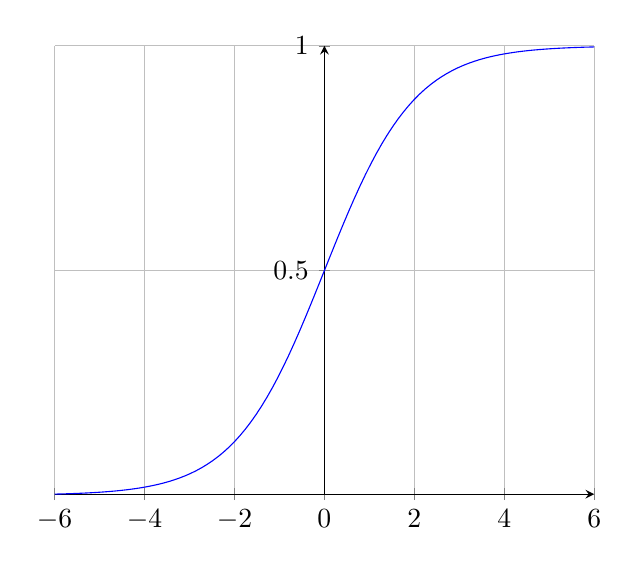
\begin{tikzpicture}
    \begin{axis}%
    [
        grid=major,     
        xmin=-6,
        xmax=6,
        axis x line=bottom,
        ytick={0,.5,1},
        ymax=1,
        axis y line=middle,
    ]
        \addplot%
        [
            blue,%
            mark=none,
            samples=100,
            domain=-6:6,
        ]
        (x,{1/(1+exp(-x))});
    \end{axis}
\end{tikzpicture}
\end{center}

Astfel, în contextul clasificării binare, vom eticheta instanța $x$ cu:

\[
y_x=
	\begin{cases}
		\text{1,} &\quad \pred \geq 0.5 \\
		\text{0,} &\quad \pred < 0.5 \\
	\end{cases}
\]

Fiind dat un set de date cu $m$ exemple $\{(x^{(1)}, y^{(1)})...(x^{(m)}, y^{(m)})\}$ dorim ca $\pred^{(i)} \approx y^{(i)}$. Vom defini, pentru o predicție, funcția de eroare: $$L(\pred, y)=-(ylog(\pred) + (1-y)log(1 - \pred))$$ și costul pentru întregul set de date este dat de: $$\displaystyle{J(w,b)=\frac{1}{m}\sum\limits_{i=1}^{m}L(\pred^{(i)}, y^{(i)})}$$

Regresia logistică este, în fapt, o problemă de optimizare, în care încercăm sa găsim o configurație cât mai bună pentru parametrii $w$ și $b$ pentru a minimiza costul $J$ pentru un anumit set de date, iar în continuare vom prezenta câțiva algoritmi care ne vor ajuta în acest sens.

\subsection{Metode de optimizare bazate pe gradient}
\subsubsection{Metoda gradientului descendent}

Acesta este un algoritm de optimizare iterativ care aproximează minimul, de cele mai multe ori cel local, a unei funcții. În contextul funcției de cost $J$ asociată regresiei logistice, algoritmul gradient descent are următorul pseudocod:

\begin{algorithm}
\caption{Gradient Descent}
\begin{algorithmic}[1]
\While {stopping condition}
\State $w = w - \alpha\frac{\partial J(w,b)}{\partial w}$
\State $b = b - \alpha\frac{\partial J(w,b)}{\partial b}$
\EndWhile
\end{algorithmic}
\end{algorithm}

Condiția de oprire poate să fie efectuarea unui număr de iterații sau neîmbunătățirea rezultatului cu o valoare mai mare decât un $\epsilon$ fixat. Din punct de vedere grafic, pașii algoritmului arată astfel:

\begin{center}
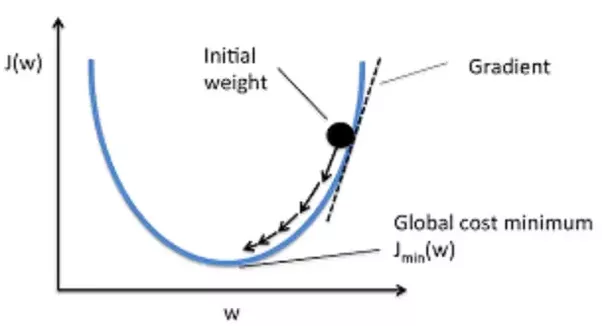
\includegraphics[scale=0.5]{gradientDescent} \\
\textit{Funcția J din figură este o variantă simplificată a celei folosită în model, ignorând parametrul b}
\end{center}

Există un așa numit hyper-parametru $\alpha$ (learning rate) care influențează mărimea pașilor efectuați atunci când algoritmul mișcă într-o direcție parametrii funcției ce trebuie minimizată. Acesta este fixat, rămâne constant pe tot parcursul execuției și valorile obișnuite sunt de ordinul $\{0.01, 0.001, 0.0001, ...\}$. Totuși, dacă folosim o valoare mare, apare riscul de a face pași prea mari și să ratăm cu totul minimul, iar dacă folosim o valoare mică, dispare acest risc, însă convergență ar necesita mult mai mult timp din cauza pașilor foarte mici.

\begin{center}
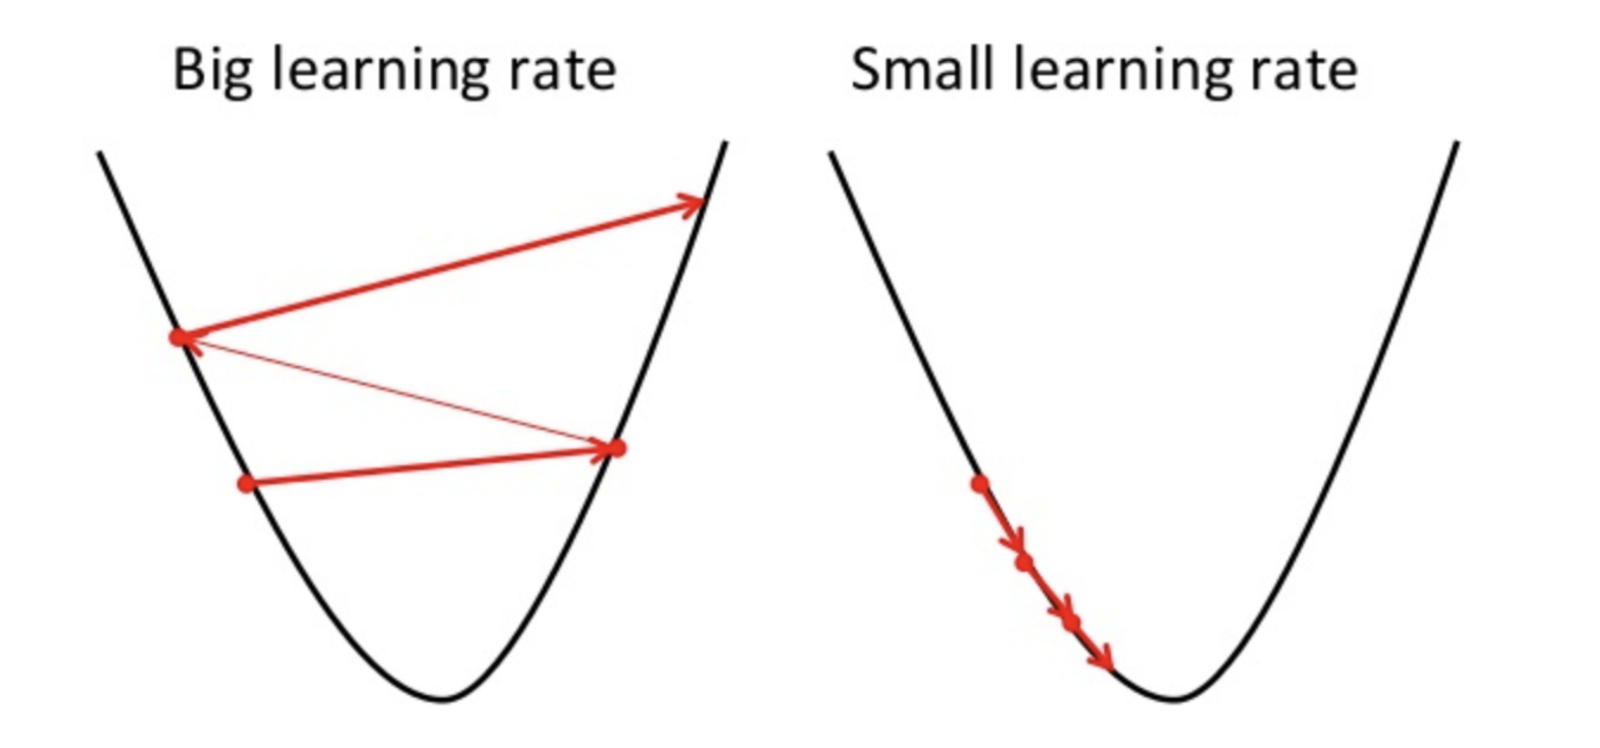
\includegraphics[scale=0.2]{gradientDescentLearningRate}
\end{center} 

Problema de optimizare din cadrul regresiei logistice este una convexă iar algoritmul Gradient Descent face o treabă bună în a minimiza costul $J$, neavând inconvenienţa minimelor locale. 

\subsubsection{Momentum}
În următoarele 3 puncte vom prezenta imbunătățiri aduse algoritmului inițial, ce au ca efect scăderea timpului necesar pentru convergență. Prima dintre aceste îmbunătățiri se numește  \textit{Momentum} și are la bază conceptul de medii ponderate exponențiale. \\

Fie un set de puncte într-un plan $\{p_0, p_2, ..., p_n\}$. Prin folosirea acestor medii, se poate aproxima eficient, un drum ce începe din $p_0$, se termină în $p_n$ și trece prin toate cele $n$ puncte.
\begin{center}
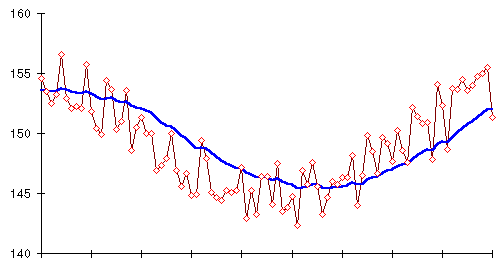
\includegraphics[scale=0.7]{expWeightedAvg} \\
\textit{Drumul complet de la } $p_0 \, la \, p_n $ \textit{(linia roșie) și drumul aproximat (linia albastră)}
\end{center}

Linia albastră este dată de următoarea regulă:

\[
v_t=
	\begin{cases}
		\text{0,} &\quad t=0 \\
		\beta v_{t-1} + (1-\beta)p_t &\quad t > 0 \\
	\end{cases}
\quad t=\overline{0,n}
\]

Aceste idei se pot implementa în cadrul algoritmului original Gradient Descent pentru a grăbi convergență astfel:

\begin{algorithm}
\caption{Gradient Descent with Momentum}
\begin{algorithmic}[2]
\State $v_{dW} = 0$
$v_{db} = 0$
\While {stopping condition}
\State $dW = \frac{\partial J(w,b)}{\partial w}$
\State $db = \frac{\partial J(w,b)}{\partial b}$
\State $v_{dW} = \beta v_{dW} + (1-\beta)dW$
\State $v_{db} = \beta v_{db} + (1-\beta)db$
\State $W = W - \alpha v_{dW}$
\State $b = b - \alpha v_{db}$
\EndWhile
\end{algorithmic}
\end{algorithm}

În acestă versiune mai apare încă un hyper-parametru $\beta$, însă acesta are valoarea 0.9 și este rar modificat.

\begin{center}
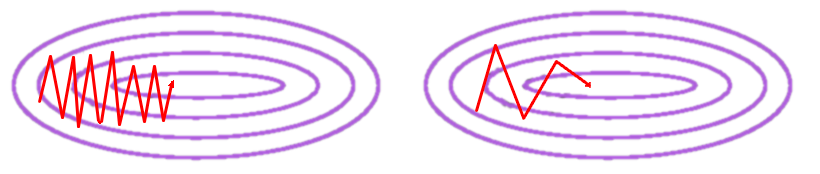
\includegraphics[scale=0.5]{momentum} \\
\textit{Pașii făcuți de algoritmul original} \quad \textit{Pașii făcuți când se folosește Momentum}
\end{center}

\subsubsection{RMSProp}

\begin{algorithm}
\caption{RMSProp}
\begin{algorithmic}[3]
\State $s_{dW} = 0$
$s_{db} = 0$
\While {stopping condition}
\State $dW = \frac{\partial J(w,b)}{\partial w}$
\State $db = \frac{\partial J(w,b)}{\partial b}$
\State $s_{dW} = \beta s_{dW} + (1-\beta)dW^2$
\State $s_{db} = \beta s_{db} + (1-\beta)db^2$
\State $\displaystyle{W = W - \alpha \frac{dW}{\sqrt{s_{dW} + \epsilon}}}$
\State $\displaystyle{b = b - \alpha \frac{db}{\sqrt{s_{db} + \epsilon}}}$
\EndWhile
\end{algorithmic}
\end{algorithm}

RMSProp își propune să micșoreze oscilațiile în direcții divergente de locația minimului, făcute de Gradient Descent, prin modificarea cu valori foarte mici a parametrilor ce duc spre direcții neoptime. \cite{rmsprop}

\subsubsection{Adam}

Adam combină Momentum și RMSProp într-un singur algoritm oferind, în majoritatea cazurilor, un rezultat mai bun decât cele 2. \cite{adam}

\begin{algorithm}
\caption{Adam}
\begin{algorithmic}[4]
\State $v_{dW} = 0$
$v_{db} = 0$
$s_{dW} = 0$
$s_{db} = 0$
\While {stopping condition}
\State On iteration $t$
\State $dW = \frac{\partial J(w,b)}{\partial w}$
$db = \frac{\partial J(w,b)}{\partial b}$
\State $v_{dW} = \beta_1 v_{dW} + (1-\beta_1)dW$
$v_{db} = \beta_1 v_{db} + (1-\beta_1)db$
\State $s_{dW} = \beta_2 s_{dW} + (1-\beta_2)dW^2$
$s_{db} = \beta_2 s_{db} + (1-\beta_2)db^2$
\State $\displaystyle{v_{dW}^{corrected} = \frac{v_{dW}}{1 - \beta_1^t}}$
$\displaystyle{v_{db}^{corrected} = \frac{v_{db}}{1 - \beta_1^t}}$
\State $\displaystyle{s_{dW}^{corrected} = \frac{s_{dW}}{1 - \beta_2^t}}$
$\displaystyle{s_{db}^{corrected} = \frac{s_{db}}{1 - \beta_2^t}}$
\State $\displaystyle{W = W - \alpha \frac{v_{dW}^{corrected}}{\sqrt{s_{dW}^{corrected} + \epsilon}}}$
$\displaystyle{b = b - \alpha \frac{v_{db}^{corrected}}{\sqrt{s_{db}^{corrected} + \epsilon}}}$
\EndWhile
\end{algorithmic}
\end{algorithm} 

În acest caz, există 3 hyper-parametrii $\alpha, \, \beta_1, \, \beta_2$. Dacă $\beta_1=0.9$ și $\beta_2=0.99$ sunt valori standardizate și foarte rar schimbate, $\alpha$ reprezintă cel mai important hyper-parametru și cel care are efectul net cel mai mare. Din această cauză, căutarea unei valori cât mai bune pentru acesta este un proces necesar pentru a obține o performanță bună.

\subsection{Rețele neuronale}
\subsubsection{Structură și notații}

\tikzset{%
  every neuron/.style={
    circle,
    draw,
    minimum size=1cm
  },
  neuron missing/.style={
    draw=none, 
    scale=4,
    text height=0.333cm,
    execute at begin node=\color{black}$\vdots$
  },
}

\begin{center}
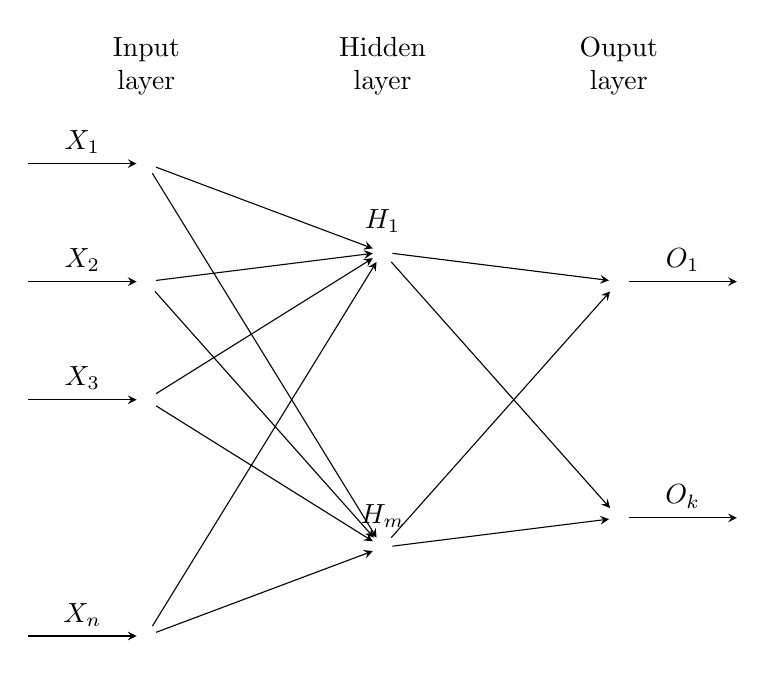
\begin{tikzpicture}[x=1.5cm, y=1.5cm, >=stealth]

\foreach \m/\l [count=\y] in {1,2,3,missing,4}
  \node [every neuron/.try, neuron \m/.try] (input-\m) at (0,2.5-\y) {};

\foreach \m [count=\y] in {1,missing,2}
  \node [every neuron/.try, neuron \m/.try ] (hidden-\m) at (2,2-\y*1.25) {};

\foreach \m [count=\y] in {1,missing,2}
  \node [every neuron/.try, neuron \m/.try ] (output-\m) at (4,1.5-\y) {};

\foreach \l [count=\i] in {1,2,3,n}
  \draw [<-] (input-\i) -- ++(-1,0)
    node [above, midway] {$X_\l$};

\foreach \l [count=\i] in {1,m}
  \node [above] at (hidden-\i.north) {$H_\l$};

\foreach \l [count=\i] in {1,k}
  \draw [->] (output-\i) -- ++(1,0)
    node [above, midway] {$O_\l$};

\foreach \i in {1,...,4}
  \foreach \j in {1,...,2}
    \draw [->] (input-\i) -- (hidden-\j);

\foreach \i in {1,...,2}
  \foreach \j in {1,...,2}
    \draw [->] (hidden-\i) -- (output-\j);

\foreach \l [count=\x from 0] in {Input, Hidden, Ouput}
  \node [align=center, above] at (\x*2,2) {\l \\ layer};

\end{tikzpicture}
\end{center}

Imaginea de mai sus reprezintă o rețea neuronală clasică și, la nivel înalt, are 3 componente principale. Un \textit{input layer}, unul sau mai multe \textit{hidden layers} și un \textit{output layer}. Informația pornește de la input către output fiind procesată pe parcurs și la baza întregii construcții se află \textit{neuronul}, reprezentat în figură prin cerc.

\begin{center}
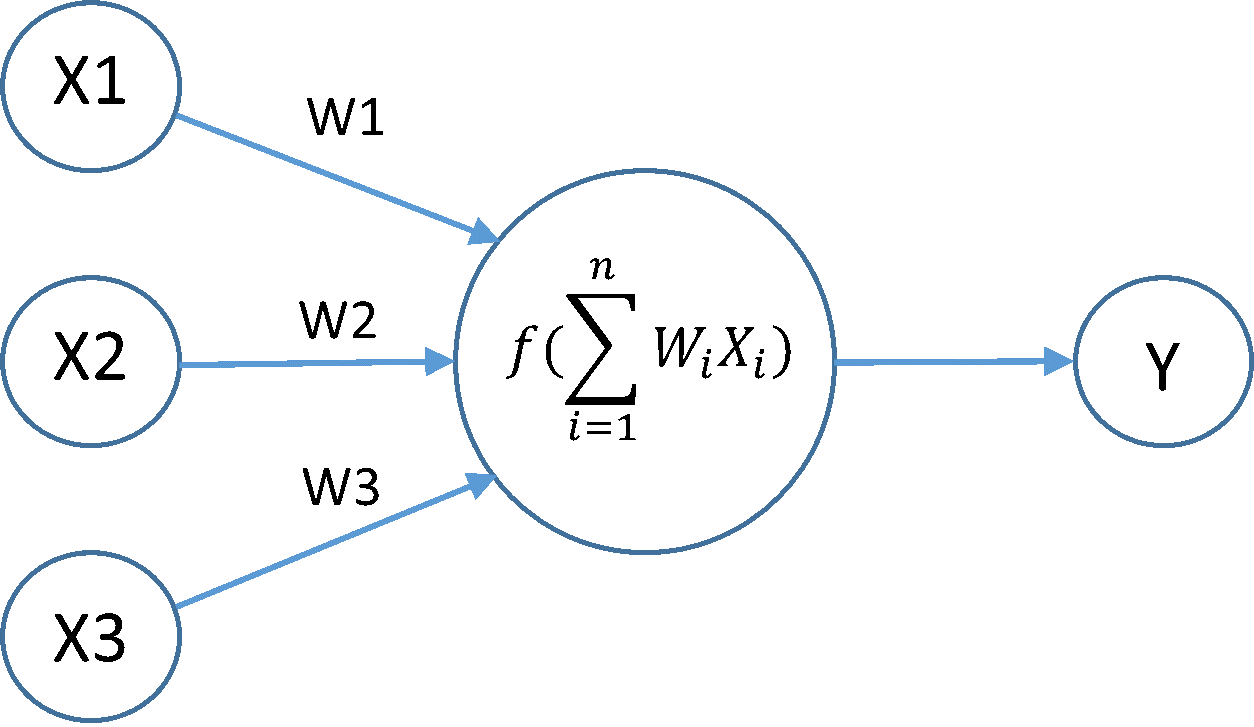
\includegraphics[scale=0.5]{neuron} \\
\textit{Un neuron}
\end{center}

Fie $x=[x_1,x_2,x_3], \; w=[w_1,w_2,w_3] \quad x,w \in \mathbb{R}^3$ și $b \in \mathbb{R}$ (omis în figură). Operațiile care se fac în cadrul unui neuron sunt:

\begin{enumerate}
\centering
\item $z=w^Tx + b$
\item $y=f(z)$
\end{enumerate}

În care vectorul \textit{w} și numărul \textit{b} sunt parametrii, \textit{x} este un vector input și \textit{y} se numește valoarea activării neuronului, \textit{f} fiind funcția de activare. \\
Se observă că dacă înlocuim $f$ cu funcția sigmoid $\displaystyle{\sigma(z)=\frac{1}{1 + e^{-z}}}$ obținem fix modelul regresiei logistice, el putând fi interpretat ca o rețea neuronală cu un singur neuron.

\subsubsection{Funcții de activare}
Am văzut cât este de simplu să obținem regresia logistică dacă înlocuim funcția de activare cu funcția sigmoid, însă există și alte opțiuni consacrate pe lângă aceasta.

\begin{enumerate}
\item \textbf{Funcția tangentă hiperbolică (Hyperbolic tangent)}: $\displaystyle{tanh(z)=\frac{e^x-e^{-x}}{e^x + e^{-x}}}$

\begin{center}
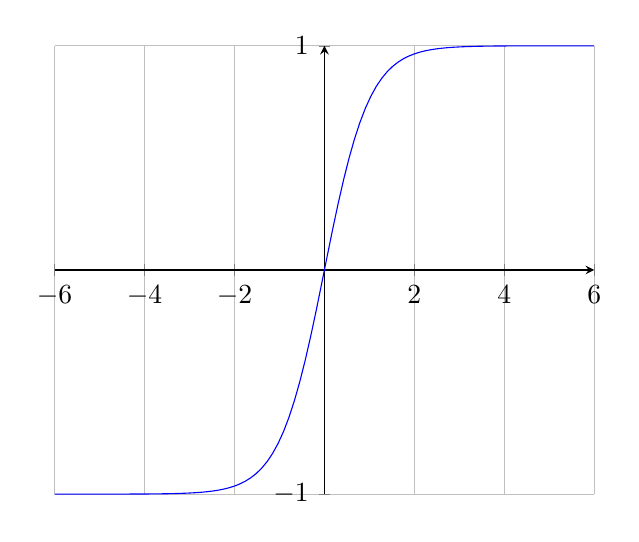
\begin{tikzpicture}
    \begin{axis}%
    [
        grid=major,     
        xmin=-6,
        xmax=6,
        axis x line=middle,
        ytick={-1,0,1},
        ymax=1,
        axis y line=middle,
    ]
        \addplot%
        [
            blue,%
            mark=none,
            samples=100,
            domain=-6:6,
        ]
        (x,{(exp(x)-exp(-x))/((exp(x)+exp(-x))});
    \end{axis}
\end{tikzpicture}
\end{center}

\item \textbf{Rectified Linear Unit (ReLU)}: $relu(z)=max(z, 0)$

\begin{center}
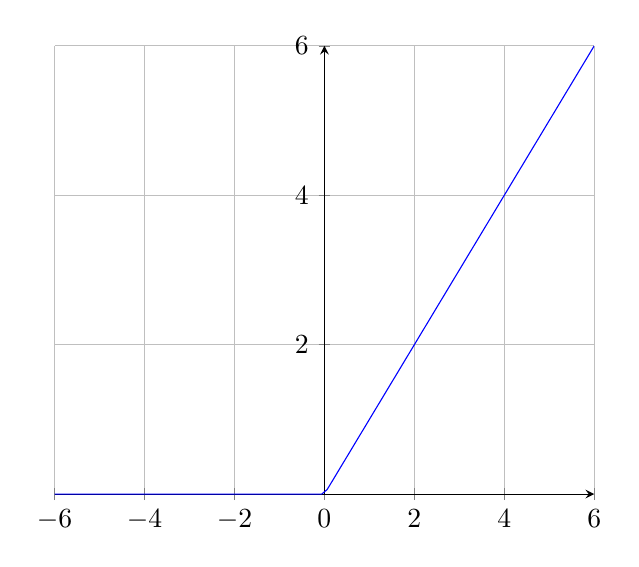
\begin{tikzpicture}
    \begin{axis}%
    [
        grid=major,     
        xmin=-6,
        xmax=6,
        axis x line=bottom,
        ytick={0,2,4,6},
        ymax=6,
        axis y line=middle,
    ]
        \addplot%
        [
            blue,%
            mark=none,
            samples=100,
            domain=-6:6,
        ]
        (x,{max(x,0)});
    \end{axis}
\end{tikzpicture}
\end{center}

\item \textbf{Leaky ReLU}: $leakyReLU(z)=max(z, 0.01z)$

\begin{center}
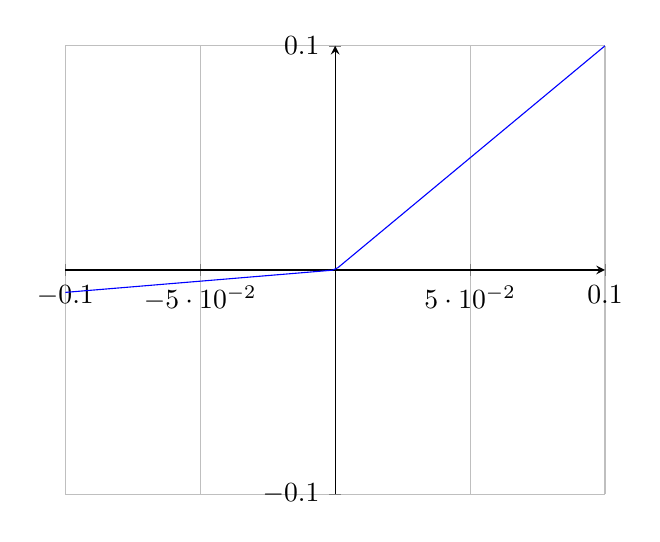
\begin{tikzpicture}
    \begin{axis}%
    [
        grid=major,     
        xmin=-0.1,
        xmax=0.1,
        axis x line=middle,
        ytick={-0.1,0,0.1,0.2},
        ymin=-0.1,
        ymax=0.1,
        axis y line=middle,
    ]
        \addplot%
        [
            blue,%
            mark=none,
            samples=100,
            domain=-0.1:0.1,
        ]
        (x,{max(x,0.1*x)});
    \end{axis}
\end{tikzpicture}
\end{center}

\end{enumerate}

\subsubsection{Propagarea înainte (Feed-Foward Propagation)}
În această secțiune vom studia operațiile ce intervin când informația parcurge traseul \textit{input-output}. Fie următoarea rețea neuronală:

\begin{center}
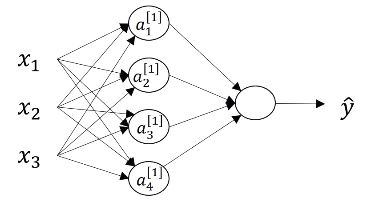
\includegraphics[scale=1]{feedFoward}
\end{center}

Modelul nostru primește ca date de intrare un vector $x \in \mathbb{R}^3$, are un \textit{hidden layer} cu 4 neuroni și va oferi ca \textit{output} un număr real. Vom folosi notațiile:

\begin{itemize}
\item $x \in \mathbb{R}^3 \rightarrow$ vector de input.

\[
x=
\begin{bmatrix}
x_1 \\
x_2 \\
x_3 \\
\end{bmatrix}
\]
 
\item $a_t^{[l]} \rightarrow$ Activarea neuronului \textit{t} din layer-ul \textit{l}.
\item $A^{[l]} \rightarrow$ Vector ce conține activările tuturor neuronilor din layer-ul \textit{l}.
\item $W^{[1]} \in M_{4,3}(\mathbb{R}) \rightarrow$ Matrice ce conține parametrii \textit{w} pentru fiecare neuron din primul layer pe câte o linie. \\

\[
W^{[1]}=
\begin{bmatrix}
    w_{11} & w_{12} & w_{13} & w_{14} \\
    w_{21} & w_{22} & w_{23} & w_{24} \\
    w_{31} & w_{32} & w_{33} & w_{34} \\
    w_{41} & w_{42} & w_{43} & w_{44}
\end{bmatrix}
\]

\item $W^{[2]} \in M_{1,4}(\mathbb{R}) \rightarrow$ Matrice ce conține parametrii \textit{w} pentru fiecare neuron din ultimul layer pe câte o linie. \\

\[
W^{[2]}=
\begin{bmatrix}
    w_{11} & w_{12} & w_{13} & w_{14}
\end{bmatrix}
\]

\item $b^{[1]} \in \mathbb{R}^4 \quad b=[b_1,b_2,b_3,b_4] \rightarrow$ vector ce reține parametrii \textit{b} pentru fiecare neuron din primul layer.

\item $b^{[2]} \in \mathbb{R} \quad b=[b_1] \rightarrow$ vector ce reține parametrii \textit{b} pentru fiecare neuron din ultimul layer.
\end{itemize}

Astfel operațiile ce se produc în propagarea $input-output$ sunt:

\begin{enumerate}
\item $A^{[0]} = x \;$ considerăm $x$ valorile de activare a layer-ului de $input$.
\item $Z^{[1]} = W^{[1]}a^{[0]} + b^{[1]}$
\item $A^{[1]} = f(z^{[1]})$
\item $Z^{[2]} = W^{[2]}a^{[1]} + b^{[2]}$
\item $A^{[2]} = f(z^{[2]})$
\item $\pred=A^{[2]}$
\end{enumerate}

$A^{[2]}$ reprezintă valoarea finală, fiind activarea layer-ului de $output$, iar $f$ este o funcție oarecare de activare. \cite{deeplearningAI}

\subsubsection{Funcția de cost}
Am văzut cum regresia logistică este o rețea neuronală foarte simplă. Datorită acestui fapt, funcția de cost folosită atunci, în cadrul clasificării binare, poate fi utilizată pentru a antrena și rețele neuronale complexe.
$$L(\pred, y)=-(ylog(\pred) + (1-y)log(1 - \pred))$$
$$\displaystyle{J(W,b)=\frac{1}{m}\sum\limits_{i=1}^{m}L(\pred^{(i)}, y^{(i)})}$$ 

\subsubsection{Propagarea înapoi (Backpropagation)}
O problemă complicată în antrenarea rețelelor neuronale este propagarea erorii ce este produsă de activarea ultimului layer, cel de $output$, către neuronii aflați la începutul rețelei. Am prezentat modul în care informația parcurge traseul $input-output$, însă, pentru optimizarea parametrilor, trebuie sa parcurgem traseul opus, $output-input$, inversând toate operațiile făcute. Pentru aceasta, vom prezenta algoritmul \textit{Backpropagation}. Fie aceeași rețea neuronală ca la \textit{Feed-Foward Propagation} și folosind aceleași notații:

\begin{center}
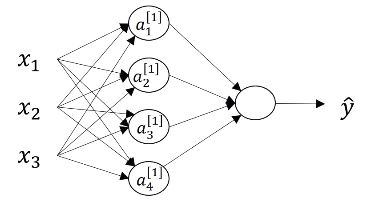
\includegraphics[scale=1]{feedFoward}
\end{center}

Operațiile efectuate de către \textit{Backpropagation} sunt:

\begin{enumerate}
\item $A^{[2]}=\pred$
\item $dZ^{[2]}=A^{[2]}-Y$
\item $\displaystyle{dW^{[2]} = \frac{1}{m}dZ^{[2]}{A^{[2]}}^T}$
\item $\displaystyle{db^{[2]} = \frac{1}{m}} np.sum(dZ^{[2]}, axis=1, keepdims=True)$ \footnote{comandă \textit{numpy} ce face suma compenentelor pentru fiecare linie (pentru un input de forma $[n,m]$ vom obține un output de forma $[n,1]$)}
\item $dZ^{[1]}={W^{[2]}}^TdZ^{[2]} * f'(Z^{[1]})$
\item $\displaystyle{dW^{[1]} = \frac{1}{m} dZ^{[1]}X^T}$
\item $\displaystyle{db^{[1]} = \frac{1}{m}} np.sum(dZ^{[1]}, axis=1, keepdims=True)$
\end{enumerate}

După execuția acestui algoritm, avem calculați 4 vector $\{dW^{[2]},db^{[2]},dW^{[1]},db^{[1]}\}$ pe care îi vom folosi pentru a modifica parametrii $W,b$ a fiecărui layer, folosind unul din algoritmii de optimizare bazați pe gradient prezentați anterior. \cite{deeplearningAI}

\subsubsection{Regularizare $L_2$ și Dropout}
În învățarea automată, o problemă frecventă este super-specializarea (overfitting) și, din păcate, aceasta este foarte întâlnită și în deep learning.

\begin{center}
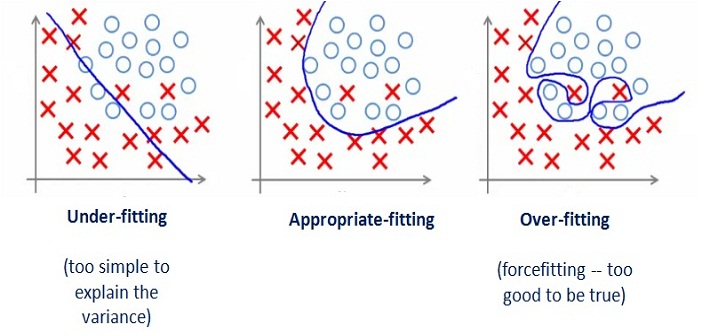
\includegraphics[scale=0.7]{fittings}
\end{center}

Pentru a ameliora acest efect nedorit, vom folosi ceea ce se numește $regularizare$, cele mai folosite 2 forme fiind:

\begin{enumerate}
\item \textbf{Regularizare $L_2$}: \\
Vom aduce o mică modificare funcției de cost inițiale:
$$\displaystyle{J(W^{[l]},b^{[l]})=\frac{1}{m}\sum\limits_{i=1}^{m}L(\pred^{(i)}, y^{(i)}) + \frac{\lambda}{2m}\sum\limits_{l=1}^{L}{\Vert W^{[l]} \Vert}_{F}^{2}}$$

$\lambda \rightarrow$ termen de regularizare \\
$L \rightarrow$ Numărul de layere din rețea 

Pentru a minimiza această funcție $J$ modificată, trebuie ca $W^{[l]} \approx 0$. Astfel, o parte din neuroni au activări mici, creându-se un model mai simplu, ce nu descrie perfect datele de antrenament, dar care are o capacitate de generalizare mai mare.

\item \textbf{Dropout}: \\
Vom fixa un hyper-parametru $keep\_prob \in [0,1]$. În fiecare iterație din procesul de antrenare, vom asocia aleatoriu fiecărui neuron o valoare în intervalul $[0,1]$. Dacă acestă valoare depășește $keep\_prob$, nu vom lua în calcul neuronul respectiv în iterația curentă, setându-i temporar activarea pe 0.

\begin{center}
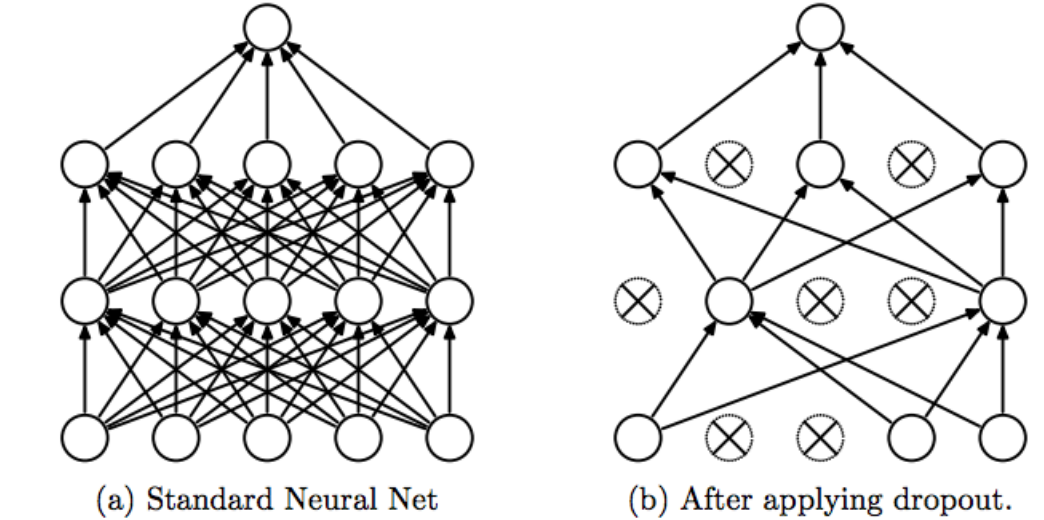
\includegraphics[scale=0.3]{dropout}
\end{center}

Efectul acestei metode este de asemenea un model mai simplu care are capacitatea de generalizare mai mare decât a celui ce descrie perfect datele de antrenament.

\end{enumerate}



